%  LaTeX support: latex@mdpi.com 
%  For support, please attach all files needed for compiling as well as the log file, and specify your operating system, LaTeX version, and LaTeX editor.

%=================================================================
\documentclass[remotesensing,article,submit,pdftex,moreauthors]{Definitions/mdpi} 

\usepackage{subcaption}


%--------------------
% Class Options:
%--------------------
%----------
% journal
%----------
% Choose between the following MDPI journals:
% acoustics, actuators, addictions, admsci, adolescents, aerobiology, aerospace, agriculture, agriengineering, agrochemicals, agronomy, ai, air, algorithms, allergies, alloys, analytica, analytics, anatomia, animals, antibiotics, antibodies, antioxidants, applbiosci, appliedchem, appliedmath, applmech, applmicrobiol, applnano, applsci, aquacj, architecture, arm, arthropoda, arts, asc, asi, astronomy, atmosphere, atoms, audiolres, automation, axioms, bacteria, batteries, bdcc, behavsci, beverages, biochem, bioengineering, biologics, biology, biomass, biomechanics, biomed, biomedicines, biomedinformatics, biomimetics, biomolecules, biophysica, biosensors, biotech, birds, bloods, blsf, brainsci, breath, buildings, businesses, cancers, carbon, cardiogenetics, catalysts, cells, ceramics, challenges, chemengineering, chemistry, chemosensors, chemproc, children, chips, cimb, civileng, cleantechnol, climate, clinpract, clockssleep, cmd, coasts, coatings, colloids, colorants, commodities, compounds, computation, computers, condensedmatter, conservation, constrmater, cosmetics, covid, crops, cryptography, crystals, csmf, ctn, curroncol, cyber, dairy, data, ddc, dentistry, dermato, dermatopathology, designs, devices, diabetology, diagnostics, dietetics, digital, disabilities, diseases, diversity, dna, drones, dynamics, earth, ebj, ecologies, econometrics, economies, education, ejihpe, electricity, electrochem, electronicmat, electronics, encyclopedia, endocrines, energies, eng, engproc, entomology, entropy, environments, environsciproc, epidemiologia, epigenomes, est, fermentation, fibers, fintech, fire, fishes, fluids, foods, forecasting, forensicsci, forests, foundations, fractalfract, fuels, future, futureinternet, futurepharmacol, futurephys, futuretransp, galaxies, games, gases, gastroent, gastrointestdisord, gels, genealogy, genes, geographies, geohazards, geomatics, geosciences, geotechnics, geriatrics, grasses, gucdd, hazardousmatters, healthcare, hearts, hemato, hematolrep, heritage, higheredu, highthroughput, histories, horticulturae, hospitals, humanities, humans, hydrobiology, hydrogen, hydrology, hygiene, idr, ijerph, ijfs, ijgi, ijms, ijns, ijpb, ijtm, ijtpp, ime, immuno, informatics, information, infrastructures, inorganics, insects, instruments, inventions, iot, j, jal, jcdd, jcm, jcp, jcs, jcto, jdb, jeta, jfb, jfmk, jimaging, jintelligence, jlpea, jmmp, jmp, jmse, jne, jnt, jof, joitmc, jor, journalmedia, jox, jpm, jrfm, jsan, jtaer, jvd, jzbg, kidneydial, kinasesphosphatases, knowledge, land, languages, laws, life, liquids, literature, livers, logics, logistics, lubricants, lymphatics, machines, macromol, magnetism, magnetochemistry, make, marinedrugs, materials, materproc, mathematics, mca, measurements, medicina, medicines, medsci, membranes, merits, metabolites, metals, meteorology, methane, metrology, micro, microarrays, microbiolres, micromachines, microorganisms, microplastics, minerals, mining, modelling, molbank, molecules, mps, msf, mti, muscles, nanoenergyadv, nanomanufacturing,\gdef\@continuouspages{yes}} nanomaterials, ncrna, ndt, network, neuroglia, neurolint, neurosci, nitrogen, notspecified, %%nri, nursrep, nutraceuticals, nutrients, obesities, oceans, ohbm, onco, %oncopathology, optics, oral, organics, organoids, osteology, oxygen, parasites, parasitologia, particles, pathogens, pathophysiology, pediatrrep, pharmaceuticals, pharmaceutics, pharmacoepidemiology,\gdef\@ISSN{2813-0618}\gdef\@continuous pharmacy, philosophies, photochem, photonics, phycology, physchem, physics, physiologia, plants, plasma, platforms, pollutants, polymers, polysaccharides, poultry, powders, preprints, proceedings, processes, prosthesis, proteomes, psf, psych, psychiatryint, psychoactives, publications, quantumrep, quaternary, qubs, radiation, reactions, receptors, recycling, regeneration, religions, remotesensing, reports, reprodmed, resources, rheumato, risks, robotics, ruminants, safety, sci, scipharm, sclerosis, seeds, sensors, separations, sexes, signals, sinusitis, skins, smartcities, sna, societies, socsci, software, soilsystems, solar, solids, spectroscj, sports, standards, stats, std, stresses, surfaces, surgeries, suschem, sustainability, symmetry, synbio, systems, targets, taxonomy, technologies, telecom, test, textiles, thalassrep, thermo, tomography, tourismhosp, toxics, toxins, transplantology, transportation, traumacare, traumas, tropicalmed, universe, urbansci, uro, vaccines, vehicles, venereology, vetsci, vibration, virtualworlds, viruses, vision, waste, water, wem, wevj, wind, women, world, youth, zoonoticdis 
% For posting an early version of this manuscript as a preprint, you may use "preprints" as the journal. Changing "submit" to "accept" before posting will remove line numbers.

%---------
% article
%---------
% The default type of manuscript is "article", but can be replaced by: 
% abstract, addendum, article, book, bookreview, briefreport, casereport, comment, commentary, communication, conferenceproceedings, correction, conferencereport, entry, expressionofconcern, extendedabstract, datadescriptor, editorial, essay, erratum, hypothesis, interestingimage, obituary, opinion, projectreport, reply, retraction, review, perspective, protocol, shortnote, studyprotocol, systematicreview, supfile, technicalnote, viewpoint, guidelines, registeredreport, tutorial
% supfile = supplementary materials

%----------
% submit
%----------
% The class option "submit" will be changed to "accept" by the Editorial Office when the paper is accepted. This will only make changes to the frontpage (e.g., the logo of the journal will get visible), the headings, and the copyright information. Also, line numbering will be removed. Journal info and pagination for accepted papers will also be assigned by the Editorial Office.

%------------------
% moreauthors
%------------------
% If there is only one author the class option oneauthor should be used. Otherwise use the class option moreauthors.

%---------
% pdftex
%---------
% The option pdftex is for use with pdfLaTeX. Remove "pdftex" for (1) compiling with LaTeX & dvi2pdf (if eps figures are used) or for (2) compiling with XeLaTeX.

%=================================================================
% MDPI internal commands - do not modify
\firstpage{1} 
\makeatletter 
\setcounter{page}{\@firstpage} 
\makeatother
\pubvolume{1}
\issuenum{1}
\articlenumber{0}
\pubyear{2023}
\copyrightyear{2023}
%\externaleditor{Academic Editor: Firstname Lastname}
\datereceived{ } 
\daterevised{ } % Comment out if no revised date
\dateaccepted{ } 
\datepublished{ } 
%\datecorrected{} % For corrected papers: "Corrected: XXX" date in the original paper.
%\dateretracted{} % For corrected papers: "Retracted: XXX" date in the original paper.
\hreflink{https://doi.org/} % If needed use \linebreak
%\doinum{}
%\pdfoutput=1 % Uncommented for upload to arXiv.org

%=================================================================
% Add packages and commands here. The following packages are loaded in our class file: fontenc, inputenc, calc, indentfirst, fancyhdr, graphicx, epstopdf, lastpage, ifthen, float, amsmath, amssymb, lineno, setspace, enumitem, mathpazo, booktabs, titlesec, etoolbox, tabto, xcolor, colortbl, soul, multirow, microtype, tikz, totcount, changepage, attrib, upgreek, array, tabularx, pbox, ragged2e, tocloft, marginnote, marginfix, enotez, amsthm, natbib, hyperref, cleveref, scrextend, url, geometry, newfloat, caption, draftwatermark, seqsplit
% cleveref: load \crefname definitions after \begin{document}

%=================================================================
% Please use the following mathematics environments: Theorem, Lemma, Corollary, Proposition, Characterization, Property, Problem, Example, ExamplesandDefinitions, Hypothesis, Remark, Definition, Notation, Assumption
%% For proofs, please use the proof environment (the amsthm package is loaded by the MDPI class).

%=================================================================
% Full title of the paper (Capitalized)
\Title{CIRRUS: Cloud Infrared Recognition and Reconstruction via UNET System}

% MDPI internal command: Title for citation in the left column
\TitleCitation{CIRRUS: Cloud Infrared Recognition and Reconstruction via UNET System}

% Author Orchid ID: enter ID or remove command
\newcommand{\orcidauthorA}{0009-0007-5504-5838} % Add \orcidA{} behind the author's name
%\newcommand{\orcidauthorB}{0000-0000-0000-000X} % Add \orcidB{} behind the author's name

% Authors, for the paper (add full first names)
\Author{K. Sommer $^{1,*}$\orcidA{}, W. Kabalan $^{2}$ and R. Brunet $^{3}$}

%\longauthorlist{yes}

% MDPI internal command: Authors, for metadata in PDF
\AuthorNames{K. Sommer, W. Kabalan, R. Brunet}

% MDPI internal command: Authors, for citation in the left column
\AuthorCitation{Sommer, K.; Kabalan, W.; Brunet, R.}
% If this is a Chicago style journal: Lastname, Firstname, Firstname Lastname, and Firstname Lastname.

% Affiliations / Addresses (Add [1] after \address if there is only one affiliation.)
\address{%
$^{1}$ \quad Laboratoire Univers et Particules de Montpellier, Université de Montpellier, CNRS, Montpellier, France; kelian.sommer@umontpellier.fr\\
$^{2}$ \quad APC, Univ Paris Diderot, CNRS/IN2P3, CEA/lrfu, Obs de Paris, Sorbonne Paris Cit´e, France; wassim.kabalan@apc.in2p3.fr\\
$^{3}$ \quad Laboratoire d’Astrophysique de Marseille, Marseille, France}
% Contact information of the corresponding author
\corres{Correspondence: kelian.sommer@umontpellier.fr}

% Current address and/or shared authorship
%\firstnote{Current address: Affiliation 3.} 
%\firstnote{These authors contributed equally to this work.}
% The commands \thirdnote{} till \eighthnote{} are available for further notes

%\simplesumm{} % Simple summary

%\conference{} % An extended version of a conference paper

% Abstract (Do not insert blank lines, i.e. \\) 
\abstract{Infrared thermal cameras provide reliable information on the atmospheric conditions. Precise delineation of clouds in the captured sky/cloud images poses a challenge due to the ambiguous outlines of the clouds. Various methodologies have been previously suggested, employing color as the distinguishing criterion for cloud identification in the visible spectral domain. In this study, we present deep-learning image classification and segmentation architectures relying on Convolutional Neural Network (CNN) and U-Net encode/decoder network named CIRRUS and optimized for long-wave infrared band images. Our findings suggest that our trained models effectively identify and derive precise cloud structure information from radiometrically calibrated images with strong viability for sustained cloud monitoring over extended durations.}
	

%A single paragraph of about 200 words maximum.
%For research articles, abstracts should give a pertinent overview of the work. We strongly encourage authors to use the following style of structured abstracts, but without headings: (1) Background: place the question addressed in a broad context and highlight the purpose of the study; (2) Methods: describe briefly the main methods or treatments applied; (3) Results: summarize the article's main findings; (4) Conclusions: indicate the main conclusions or interpretations. The abstract should be an objective representation of the article, it must not contain results which are not presented and substantiated in the main text and should not exaggerate the main conclusions.}

% Keywords
\keyword{ground-based cloud observation; thermal-infrared camera; cloud detection; deep-learning; image segmentation and classification; convolutional neural network; u-net} 

% The fields PACS, MSC, and JEL may be left empty or commented out if not applicable
%\PACS{J0101}
%\MSC{}
%\JEL{}

%%%%%%%%%%%%%%%%%%%%%%%%%%%%%%%%%%%%%%%%%%
% Only for the journal Diversity
%\LSID{\url{http://}}

%%%%%%%%%%%%%%%%%%%%%%%%%%%%%%%%%%%%%%%%%%
% Only for the journal Applied Sciences
%\featuredapplication{Authors are encouraged to provide a concise description of the specific application or a potential application of the work. This section is not mandatory.}
%%%%%%%%%%%%%%%%%%%%%%%%%%%%%%%%%%%%%%%%%%

%%%%%%%%%%%%%%%%%%%%%%%%%%%%%%%%%%%%%%%%%%
% Only for the journal Data
%\dataset{DOI number or link to the deposited data set if the data set is published separately. If the data set shall be published as a supplement to this paper, this field will be filled by the journal editors. In this case, please submit the data set as a supplement.}
%\datasetlicense{License under which the data set is made available (CC0, CC-BY, CC-BY-SA, CC-BY-NC, etc.)}

%%%%%%%%%%%%%%%%%%%%%%%%%%%%%%%%%%%%%%%%%%
% Only for the journal Toxins
%\keycontribution{The breakthroughs or highlights of the manuscript. Authors can write one or two sentences to describe the most important part of the paper.}

%%%%%%%%%%%%%%%%%%%%%%%%%%%%%%%%%%%%%%%%%%
% Only for the journal Encyclopedia
%\encyclopediadef{For entry manuscripts only: please provide a brief overview of the entry title instead of an abstract.}

%%%%%%%%%%%%%%%%%%%%%%%%%%%%%%%%%%%%%%%%%%
% Only for the journal Advances in Respiratory Medicine
%\addhighlights{yes}
%\renewcommand{\addhighlights}{%

%\noindent This is an obligatory section in “Advances in Respiratory Medicine”, whose goal is to increase the discoverability and readability of the article via search engines and other scholars. Highlights should not be a copy of the abstract, but a simple text allowing the reader to quickly and simplified find out what the article is about and what can be cited from it. Each of these parts should be devoted up to 2~bullet points.\vspace{3pt}\\
%\textbf{What are the main findings?}
% \begin{itemize}[labelsep=2.5mm,topsep=-3pt]
% \item First bullet.
% \item Second bullet.
% \end{itemize}\vspace{3pt}
%\textbf{What is the implication of the main finding?}
% \begin{itemize}[labelsep=2.5mm,topsep=-3pt]
% \item First bullet.
% \item Second bullet.
% \end{itemize}
%}

%%%%%%%%%%%%%%%%%%%%%%%%%%%%%%%%%%%%%%%%%%
\begin{document}

%%%%%%%%%%%%%%%%%%%%%%%%%%%%%%%%%%%%%%%%%%

\section{Introduction}

Accurate and continuous monitoring of cloud properties contributes to a profound understanding of atmospheric processes, radiative interactions, and their subsequent impacts on various Earth systems.
It provides essential insights into the Earth's complex energy balance, weather patterns, and climate dynamics. Ground-based observations have long been an integral means of studying cloud formations; however, the advancement of technology has ushered in a new era of observation methodologies. In particular, the utilization of infrared thermal cameras has emerged as a promising avenue for cloud investigations. These cameras enable non-intrusive measurements of cloud temperature or radiance distributions, offering a unique perspective on cloud structures, dynamics, and their interaction with the surrounding environment. Uncooled infrared microbolometers array sensors working in the 10-12 $\mu m$ spectral band can directly detect the LWIR emission of both clouds and the atmospheric background, excluding the scattered light of the sun or starlight. Contrary to cameras operating in the visible spectrum, these LWIR sensors are able to provide reliable measurements of cloud properties at night. It makes them particularly useful for astronomical applications, to determine the cloud cover fraction during operations and therefore assess the quality of scientific observations.

Multiple ground-based all-sky and narrow field-of-view (FOV) infrared instruments have demonstrated reliable measurements of cloud properties. For example, the infrared cloud imager (ICI), can detect clouds and assess cloud coverage both in daylight and at nighttime [25]. The ICI functions as a passive instrument, measuring the downward atmospheric radiance through a relatively narrow field of view (FOV) measuring about 250 deg$^{2}$ at a resolution of 320 × 240 pixels. The all-sky infrared visible analyzer (ASIVA) [28,29] represents a distinctive device capable of acquiring an extensive field of view (FOV) infrared sky image without the need for a scanning mechanism. Nonetheless, due to its intricate structural configuration, ASIVA incurs substantial costs. The ASC-200 system combines information from two all-sky cameras facing the sky operating in both the visible spectrum (450-650 nm) and the LWIR band (8-14 $\mu m$). The latter  component is the all-sky thermal infrared visible analyzer (TIRASVC). It features a thermal microbolometer array sensitive to radiation in the 8–14 $\mu m$ spectral range and a specifically designed wide-angle germanium lens. The resolution of is 640 $\times$ 512 pixels with a 160 degrees FOV.

In this study, we use a similar infrared sensor with a narrower FOV (i.e. 60 mm F1.25 germanium athermal lens) that aims to monitor a high-sensivity photometric telescope line of sight for astronomical purposes. It is part of the StarDICE metrology experiment that aims at measuring CALSPEC spectrophotometric reference stars flux at the 0.1\% relative uncertainty level. Near-perfect or well understood atmospheric conditions are required to reach the target sensitivity. As a first step, basic indication of the atmosphere conditions in the telescope FOV provides valuable insights onto the quality of spectrophotometric measurements. In order to determine if clouds are present in infrared images, we must develop an algorithm capable of detecting them automatically. Previous work showed the capability of detecting 0.07 $W/m^{2}/sr$ difference at 1-$\sigma$ level on any pixel of the FPA. However, detecting cloud structures in the images is challenging because of their variety of shapes and radiometric flux levels. Consequently, we develop two sequential methods to: (i) classify images (e.g, detect if any cloud is present onto the image); (ii) identify cloud structure (e.g., generate a probabilistic map). The majority of related works in cloud segmentation algorithms focus on visible colored RGB images. CloudSegNet is one such example of a light-weight deep-learning encoder/decoder network that detects clouds onto daytime and nighttime visible color images. None of the proposed models have been designed for infrared thermal images containing only a single color channel as many of them rely on red and blue channels. Our goal is to propose a deep-learning architecture specifically designed for gray scaled images.

In this paper, we propose a deep-learning architecture called CIRRUS for Cloud Infrared Recognition and Reconstruction via UNET System. It is composed of two separate deep-learning models for classification based on standard Convolutional Neural Network (CNN) and U-Net encode/decoder network (e.g, consisting of convolution, deconvolution and pooling layers) for cloud structure identification. It provides a pixel-level binary labels which classes each image as either cloudy or cloud-free and a pixel-based semantic segmentation of images in the form of a probability map.

The remainder of the paper is organized as follows. The experimental setup and data acquisition procedure are detailed in Section 2. Model architectures principles and algorithms of cloud identification and structure detection are described in Section 3. Results and relevant discussions are presented in Section 4. Section 5 shows a summary of the conclusions.

\section{Model architectures}

In this section, we outline the architectural designs of two distinct deep-learning models tailored for cloud-related tasks: cloud classification using Convolutional Neural Networks (CNN) and cloud structure detection via the U-Net model. Both architectures are implemented in \textsc{Python} with the \textsc{keras}\footnote{\url{https://keras.io}} subpackage of \textsc{TensorFlow}\footnote{\url{https://www.tensorflow.org}} framework\footnote{The code developed in this paper is freely available online at \url{https://github.com/Soumyabrata/CloudSegNet}.}. Images are normalized and binned into a fixed 160 $\times$ 128 resolution format to speed up computations. Models are trained over 500 and 1000 epochs respectively using the ADAM optimizer. We use batch of 16 images with dynamic learning rate of 0.001 that decreases through the training epochs. Hyperparameters are fine tuned with the \textsc{optuna}\footnote{\url{https://optuna.org/}} hyperparameter optimization framework.

\subsection{Image classification}

Our classification model architecture consits of a Convolutional Neural Network (CNN) architecture for the purpose of distinguishing between infrared images containing clouds and those that are cloud-free. The CNN architecture consists of multiple layers designed to extract and learn relevant features from the input images. The model commences with a series of convolutional layers, each followed by rectified linear unit (ReLU) activation and max-pooling operations. This configuration facilitates the extraction of hierarchical features that are pivotal for accurate classification.

The output of the convolutional layers is then flattened and fed into fully connected layers, culminating in a final softmax layer for cloud classification. To prevent overfitting, dropout layers are strategically incorporated during training. The model is trained on a comprehensive dataset encompassing both cloud and cloud-free infrared images, with corresponding ground truth labels. The categorical cross-entropy loss function is employed for optimization, aiming to minimize the discrepancy between predicted and actual classifications.

\begin{figure}[H]
	\includegraphics[width=\hsize]{figures/FLOWCHARTS_DL_IR.pdf}
	\caption{
		Schematic diagram of the U-net encoder/decoder model architecture to identify cloud structures. Boxes represent cross-sections of square feature maps. Each map's dimensions are indicated on its lower left, and its number of channels are indicated above it. Half-grey boxes represent maps for which half of their channels are copied. The input image is a 160 × 128 radiometrically calibrated grayscale image of the sky from the LWIR instrument. Classifier model output is a boolean. Arrows represent operations, specified by the legend-notably, blue arrows represent convolutions, while gray ones represent copying (skip connections). Tensor dimensions at the output of each block are specified.  \label{fig1}}
	\end{figure}
	\unskip

\subsection{Image segmentation}

For cloud structure identification, the U-Net architecture is adopted owing to its effifiency in semantic segmentation tasks. The U-Net model comprises an encoder and a decoder, facilitating the capturing of context-rich features and precise delineation of cloud structures. The encoder integrates convolutional and max-pooling layers to progressively downsample the input image, thereby capturing high-level features. These features are then decoded using up-convolutions and skip connections, enabling the reconstruction of the segmented cloud structures. Figure \ref{} shows the architecture of the model.

\begin{figure}[H]
	
\includegraphics[width=10.5 cm]{Definitions/logo-mdpi}
	\caption{
		Schematic diagram of the U-net encoder/decoder model architecture to identify cloud structures. Boxes represent cross-sections of square feature maps. Each map's dimensions are indicated on its lower left, and its number of channels are indicated above it. Half-grey boxes represent maps for which half of their channels are copied. The input image is a 160 × 128 radiometrically calibrated grayscale image of the sky from the LWIR instrument. The output image is a probabilistic mask prediction of pixels being cloudy or clear. Arrows represent operations, specified by the legend-notably, blue arrows represent convolutions, while gray ones represent copying (skip connections). 	Tensor dimensions at the output of each block are specified. Classifier model output is a boolean. \label{fig1}}
	\end{figure}
	\unskip

\subsubsection{Encoder block}

The encoder block of CIRRUS identification model consists of four convolution layers and four max-pooling layers. We feed a normalized and binned 4x4 radiometrically calibrated image of a fixed input size (160 × 128 pixels) into the model.
The initial convolutional layer applies a set of learnable filters to the input image, extracting low-level features. Additional convolutional layers increase the complexity of learned features by applying convolutions to the feature map generated by the previous layer, creating a hierarchy of increasingly abstract features. After a set of convolutional layers, a max-pooling layer is applied to downsample the feature map. Max-pooling helps to reduce the spatial dimensions of the feature map while retaining the most salient information.

\subsubsection{Decoder block}

The decoder takes the high-level features generated by the encoder and aims to restore the spatial resolution of the original input image. In the U-Net architecture, the decoder is connected to the encoder via skip connections, enabling the network to combine local and contextual information. The decoder starts with an upsampling operation to increase the spatial dimensions of the feature map. A skip connection connects the upsampled feature map from the decoder with the corresponding feature map from the encoder. This enables the network to leverage both local and global context information. Following the concatenation, a series of convolutional layers are applied. These layers refine the combined feature map, gradually transitioning from abstract features to more detailed information. The final convolutional layer produces the segmentation mask of the U-Net model.

\subsubsection{Loss function}

The U-Net model is trained on labeled datasets containing infrared images with pixel-wise cloud structure annotations. The loss function employed for training is typically the binary cross-entropy, which quantifies the difference between predicted probabilities and actual binary class labels for each instance in the dataset. Mathematically, given an instance's true binary label $y$ (0 or 1) and the predicted probability $p$ of it belonging to class 1, the binary cross-entropy loss $\mathcal{L}$ is calculated as:
\begin{equation}
	\mathcal{L} = -\frac{1}{N}\sum_i y_i\cdot\log\left(f_w(x_i)\right) + (1-y_i)\cdot\log\left(1-f_w(x_i)\right)
\end{equation}
where $\mathcal{L}$ is the binary cross-entropy loss. $N$ is the total number of instances in the dataset, $i$ index represents an individual instance, $y_{i}$ is the $i$-th true binary label (0 or 1) and $f_w(x_i)$ is the predicted probability that belongs to class 1, based on the model with parameters $w$.
The goal of training is to minimize this loss function by adjusting the model parameters weights $w$ to better align the predicted probabilities $f_w(x_i)$ with the true labels $y_{i}$.

\subsubsection{Model output}

The output the classifier is a boolean representing whether the image contains cloud or not. On the contrary, the image segmentation model output is a probability mask that assigns a probability value to individual pixels, indicating their potential belonging in the cloud category.
 %Subsequently, a straightforward thresholding technique is applied to transform the probability mask into a binary map. The threshold for labeling is obtained from the Receiver Operating Curve (ROC) analysis specific to our experimental conditions.

\section{Experimental setup and dataset}

\subsection{Description of the instrument}

Our instrument is a FLIR Tau2 infrared thermal camera operating in the 8-14 $\mu m$ LWIR band. It consists of a focal plane array (FPA) of 640 $\times$ 512 uncooled microbolometers with 9 Hz framerate. The sensor is coupled with a narrow FOV thanks to the 60 mm F1.25 lens. The major goal of installing it on the equatorial table next to the photometric telescope of the StarDICE experiment is to evaluate sky conditions in the visible CCD camera line of sight at any instant during observations. With careful calibration, radiative transfer and simulations data analysis, we can extract useful properties of the sky to assess the atmospheric condition in real-time. Figure \ref{} shows the instrument mounted with the required controlling equipment onto the equatorial table facing the zenith inside the observatory dome. Surrounding and camera internal temperatures are monitored in real-time to correct for temperature-dependent fluctuations of the sensor response. Device control/command and image acquisition is done with the ThermalCapture ThermalGrabber USB 2.0\footnote{\url{https://thermalcapture.com/thermalcapture-grabber-usb-2-0-documents/}} interface allowing makes access to full 14-bit radiometric raw data. We develop an in-house \texttt{Python} program to control functionalities and grab images from the camera available on GitHub in open-access\footnote{\url{https://github.com/Kelian98/tau2_thermalcapture}}. Images are written into \texttt{FITS} files. An improved flat-field calibration source is positioned at regular intervals of $\approx$ 30 seconds to correct for anisotropies in pixel responses to due fixed pattern noise (FPN). True scene radiances are computed from raw images with per pixel calibration coefficient matrices (see \ref{}).

\begin{figure}
    \centering
    
    \begin{subfigure}[b]{0.4\textwidth}
        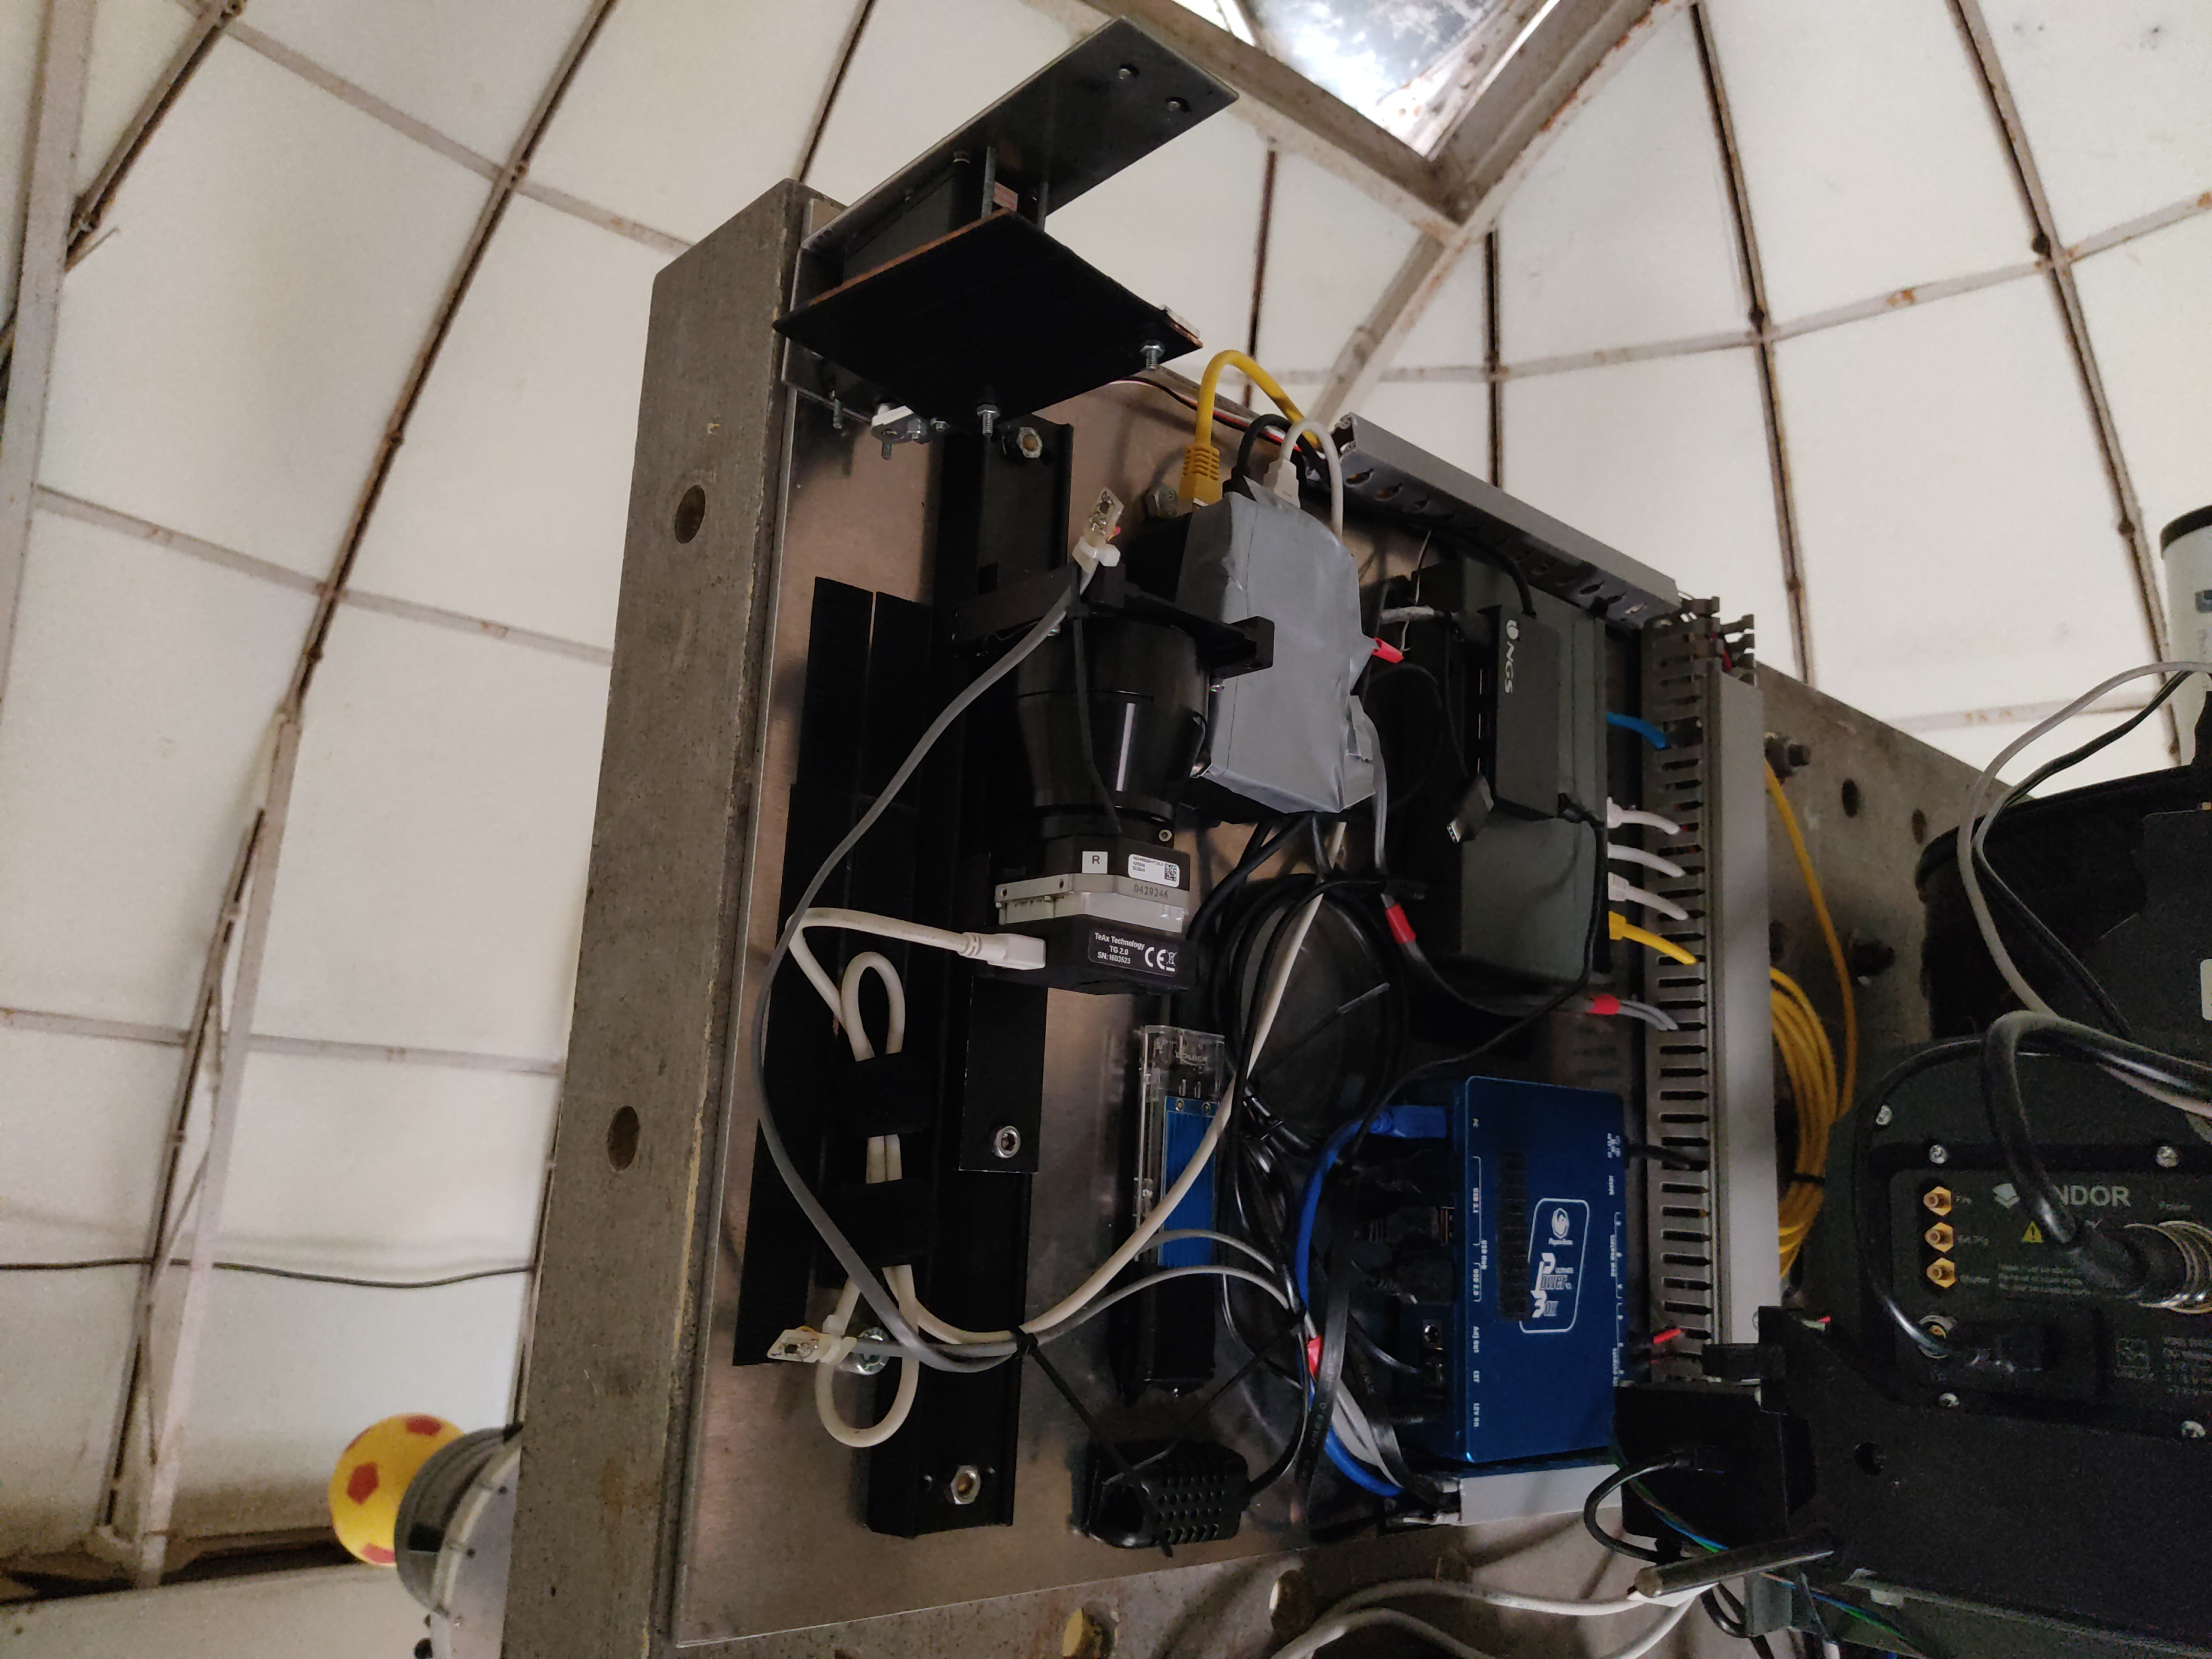
\includegraphics[width=\textwidth]{figures/infrared_instrument.jpg}
        %\caption{Subfigure 1}
        \label{fig:subfig1}
    \end{subfigure}
    \hfill
    \begin{subfigure}[b]{0.5\textwidth}
        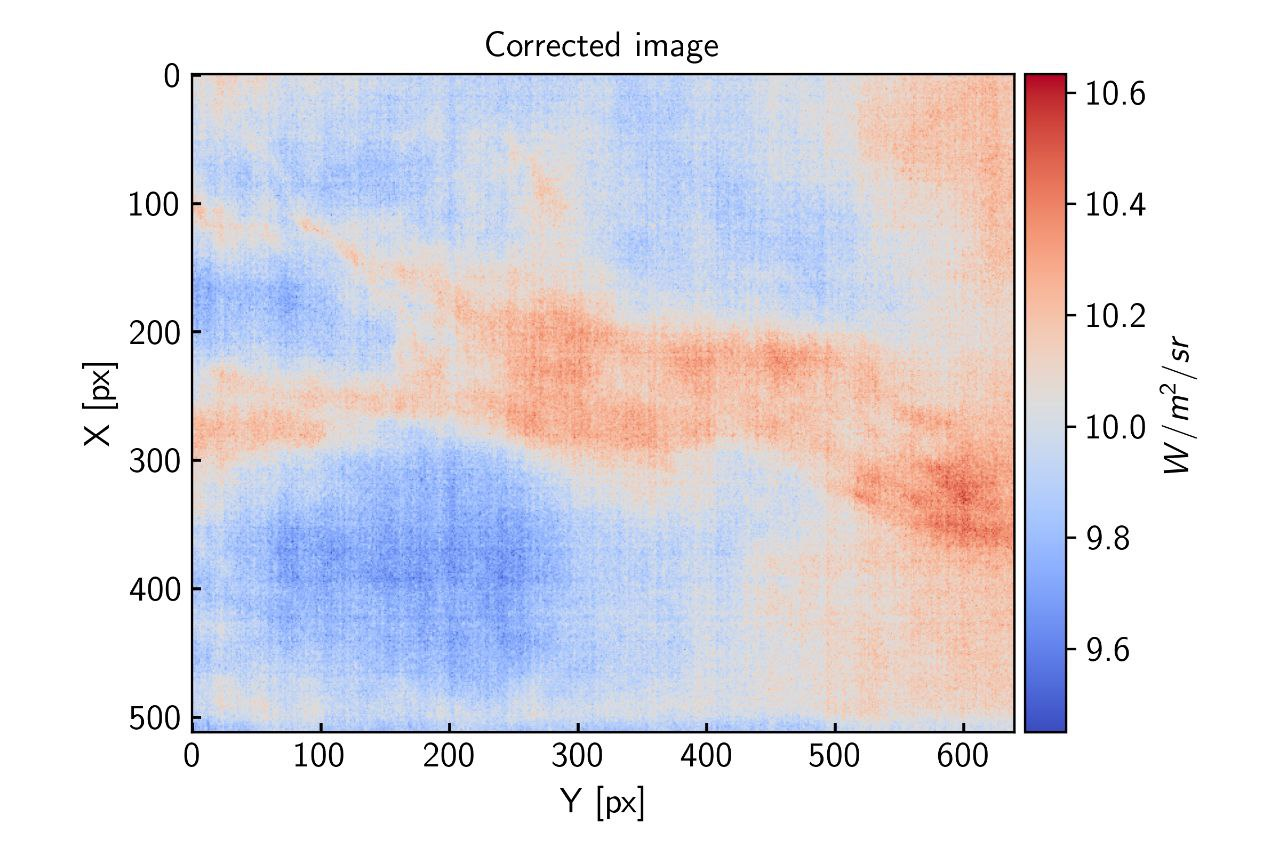
\includegraphics[width=\textwidth]{figures/calibrated_sky_image.jpg}
        %\caption{Subfigure 2}
        \label{fig:subfig2}
    \end{subfigure}
    
    \caption{\textit{Left:} infrared instrument installed onto the equatorial table of the StarDICE experiment at Observatoire de Haute-Provence. \textit{Right:} sample of radiometrically calibrated image.}
    \label{fig:side_by_side}
\end{figure}


\subsection{Extraction of sky/cloud data from LWIR images}

Infrared radiation has been recognized as holding significant promise in yielding valuable insights into cloud properties and atmospheric information. The 8–14 $\mu m$ spectral range - specifically the 10-12 $\mu m$ sometimes called the \textit{transparency window} - is characterized by minimal atmospheric emission and absorption. Radiative simulations of the atmosphere with \textsc{libRadTran} can provide a clearer depiction of the atmospheric window's attributes (e.g, sky downwelling radiance spectrum, transmittance, emittance). Figure \ref{} illustrates one typical simulation with different atmosphere reference models in the LWIR. Curves may be shifted up or down as a function of the zenith angle $\theta_{z}$, the total quantity of ozone $O_{3}$, the precipitable water vapor (PWV) or the vertical aerosol optical depth (VAOD). We can denote high atmospheric transmittance and low atmospheric emission, apart from a region around 9.6 $\mu m$ due to ozone (O3) absorption.

Sky radiance emitted by the atmosphere is primarily controlled by water vapor content and clouds. During clear-sky/cloud-free conditions, the radiation received at the ground is both minimal and subject to fluctuations based on the quantity of water vapor present. Previous investigations have demonstrated a quadratic relationship between downwelling infrared radiation and the amount of precipitable water vapor (PWV). 

\subsection{Dataset}

Cloudy and clear sky images were collected over a period of 3 nights at Observatoire de Haute-Provence in January 2023 (31◦ 24 0 N, 121 270 E) to form a composite dataset designed to train both models. The dataset consists of 20,848 cloud images and 11,000 clear-sky images. Raw analog-to-digital unit (ADU) images were transformed into true scene radiance with the calibration experiment described in \cite{}.
For the classification model, due to the imbalance of the composite dataset, 5,000 images were randomly selected from each dataset. For the segmentation model, only manually identified cloud images were selected for the training process. All images and masks are visually inspected. Samples presenting artifacts such as tree branches or building in the corner FOV are discarded. Ground-truth masks identifying cloud structure on cloud images were manually created through multiple steps of stretching procedures using \textsc{astropy} methods. They consist of boolean 2D array of the same image size, where \textit{True} identified pixels represent cloud pixels and \textit{False} identified pixels represent clear sky areas. This step could not be automated as cloud optical depths differ significantly. Indeed, the segmentation model aims at automating this tedious time consuming operation in real-time during observations. Figure \ref{} depicts two raw images with their associated manually generated ground-truth cloud masks for training purposes.

As the camera acquisition framerate enables to record up to 9 images per second, the pre-processing algorithm included constraints on consecutive image selection based on their timeseries. Selected frames are taken from at least 2 seconds between each other. Moreover, we performed multiple random augmentations (e.g, flip, shear, rotate, shift and zoom) on each original image to double the size of each dataset. All augmented images are produced through the random sequential applications of these five distinct operations to initial images. After the selection and augmentation procedures, we conducted a visual examination of all the created sky/cloud images to ensure that they appear realistic. Since all the parameters in the image augmentation process undergo controlled adjustments, our generated images closely mirror authentic sky/cloud scenes.


\section{Results}

\subsection{Loss-trend of CIRRUS}

We use this augmented composite datasets of 10,000 images respectively to train the classifier and identifer. Random sampling is applied on each composite dataset, and standard train-test-validation split is perormed in the ratio of 70\%, 20\% and 10\% respectively. Figure \ref{} depicts trends for the binary cross-entropy losses for training and testing subsets with various hyperparameters. \textsc{Optuna} framework allows ease of hyperparameters optimization. We observe that the loss saturates after a few hundred iterations for all attempts, and the model exhibits comparable loss performance for both training and testing sets. We select the model and layer parameters with the lowest validation loss for our subsequent experiments.

\subsection{Performance}

We use multiple quantitative metrics to evaluate our segmentation model : completeness, purity, Intersection over Union (IoU), precision, recall, F-score and Error Rate between the ground-truths and the predictions.

\begin{table}[H] 
	\caption{Global performance metrics on the classification and segmentation models.\label{tab1}}
	\newcolumntype{C}{>{\centering\arraybackslash}X}
	\begin{tabularx}{\textwidth}{CCC}
	\toprule
	\textbf{Title 1}	& \textbf{Title 2}	& \textbf{Title 3}\\
	\midrule
	Entry 1		& Data			& Data\\
	Entry 2		& Data			& Data \textsuperscript{1}\\
	\bottomrule
	\end{tabularx}
	\noindent{\footnotesize{\textsuperscript{1} Tables may have a footer.}}
\end{table}

Results are summarized in Table \ref{}. The purity is also
very high, with a value of 98.5. For classificatoin, the model reaches high performance of XXX accuracy and XXX YYY. We measure a completeness of 87 and a purity of 93.6. Our cloud structure identification model reaches an IoU above 0.8 at any magnitude, and up to 0.9 for bright objects (small magnitude).

\subsection{Discussion}

 

\subsection{Figures, Tables and Schemes}

All figures and tables should be cited in the main text as Figure~\ref{fig1}, Table~\ref{tab1}, etc.





The text continues here (Figure~\ref{fig2} and Table~\ref{tab2}).

% Example of a figure that spans the whole page width. The same concept works for tables, too.
\begin{figure}[H]
\begin{adjustwidth}{-\extralength}{0cm}
\centering

\includegraphics[width=15.5cm]{Definitions/logo-mdpi}
\end{adjustwidth}
\caption{This is a wide figure.\label{fig2}}
\end{figure}  

\begin{table}[H]
\caption{This is a wide table.\label{tab2}}
	\begin{adjustwidth}{-\extralength}{0cm}
		\newcolumntype{C}{>{\centering\arraybackslash}X}
		\begin{tabularx}{\fulllength}{CCCC}
			\toprule
			\textbf{Title 1}	& \textbf{Title 2}	& \textbf{Title 3}     & \textbf{Title 4}\\
			\midrule
\multirow[m]{3}{*}{Entry 1 *}	& Data			& Data			& Data\\
			  	                   & Data			& Data			& Data\\
			             	      & Data			& Data			& Data\\
                   \midrule
\multirow[m]{3}{*}{Entry 2}    & Data			& Data			& Data\\
			  	                  & Data			& Data			& Data\\
			             	     & Data			& Data			& Data\\
                   \midrule
\multirow[m]{3}{*}{Entry 3}    & Data			& Data			& Data\\
			  	                 & Data			& Data			& Data\\
			             	    & Data			& Data			& Data\\
                  \midrule
\multirow[m]{3}{*}{Entry 4}   & Data			& Data			& Data\\
			  	                 & Data			& Data			& Data\\
			             	    & Data			& Data			& Data\\
			\bottomrule
		\end{tabularx}
	\end{adjustwidth}
	\noindent{\footnotesize{* Tables may have a footer.}}
\end{table}

%\begin{listing}[H]
%\caption{Title of the listing}
%\rule{\columnwidth}{1pt}
%\raggedright Text of the listing. In font size footnotesize, small, or normalsize. Preferred format: left aligned and single spaced. Preferred border format: top border line and bottom border line.
%\rule{\columnwidth}{1pt}
%\end{listing}

Text.

Text.

\subsection{Formatting of Mathematical Components}

This is the example 1 of equation:
\begin{linenomath}
\begin{equation}
a = 1,
\end{equation}
\end{linenomath}
the text following an equation need not be a new paragraph. Please punctuate equations as regular text.
%% If the documentclass option "submit" is chosen, please insert a blank line before and after any math environment (equation and eqnarray environments). This ensures correct linenumbering. The blank line should be removed when the documentclass option is changed to "accept" because the text following an equation should not be a new paragraph.

This is the example 2 of equation:
\begin{adjustwidth}{-\extralength}{0cm}
\begin{equation}
a = b + c + d + e + f + g + h + i + j + k + l + m + n + o + p + q + r + s + t + u + v + w + x + y + z
\end{equation}
\end{adjustwidth}

% Example of a page in landscape format (with table and table footnote).
%\startlandscape
%\begin{table}[H] %% Table in wide page
%\caption{This is a very wide table.\label{tab3}}
%	\begin{tabularx}{\textwidth}{CCCC}
%		\toprule
%		\textbf{Title 1}	& \textbf{Title 2}	& \textbf{Title 3}	& \textbf{Title 4}\\
%		\midrule
%		Entry 1		& Data			& Data			& This cell has some longer content that runs over two lines.\\
%		Entry 2		& Data			& Data			& Data\textsuperscript{1}\\
%		\bottomrule
%	\end{tabularx}
%	\begin{adjustwidth}{+\extralength}{0cm}
%		\noindent\footnotesize{\textsuperscript{1} This is a table footnote.}
%	\end{adjustwidth}
%\end{table}
%\finishlandscape


Please punctuate equations as regular text. Theorem-type environments (including propositions, lemmas, corollaries etc.) can be formatted as follows:
%% Example of a theorem:
\begin{Theorem}
Example text of a theorem.
\end{Theorem}

The text continues here. Proofs must be formatted as follows:

%% Example of a proof:
\begin{proof}[Proof of Theorem 1]
Text of the proof. Note that the phrase ``of Theorem 1'' is optional if it is clear which theorem is being referred to.
\end{proof}
The text continues here.

%%%%%%%%%%%%%%%%%%%%%%%%%%%%%%%%%%%%%%%%%%
\section{Discussion}

Authors should discuss the results and how they can be interpreted from the perspective of previous studies and of the working hypotheses. The findings and their implications should be discussed in the broadest context possible. Future research directions may also be highlighted.

%%%%%%%%%%%%%%%%%%%%%%%%%%%%%%%%%%%%%%%%%%
\section{Conclusions}

This section is not mandatory, but can be added to the manuscript if the discussion is unusually long or complex.

%%%%%%%%%%%%%%%%%%%%%%%%%%%%%%%%%%%%%%%%%%
\section{Patents}

This section is not mandatory, but may be added if there are patents resulting from the work reported in this manuscript.

%%%%%%%%%%%%%%%%%%%%%%%%%%%%%%%%%%%%%%%%%%
\vspace{6pt} 

%%%%%%%%%%%%%%%%%%%%%%%%%%%%%%%%%%%%%%%%%%
%% optional
%\supplementary{The following supporting information can be downloaded at:  \linksupplementary{s1}, Figure S1: title; Table S1: title; Video S1: title.}

% Only for journal Methods and Protocols:
% If you wish to submit a video article, please do so with any other supplementary material.
% \supplementary{The following supporting information can be downloaded at: \linksupplementary{s1}, Figure S1: title; Table S1: title; Video S1: title. A supporting video article is available at doi: link.}

% Only for journal Hardware:
% If you wish to submit a video article, please do so with any other supplementary material.
% \supplementary{The following supporting information can be downloaded at: \linksupplementary{s1}, Figure S1: title; Table S1: title; Video S1: title.\vspace{6pt}\\
%\begin{tabularx}{\textwidth}{lll}
%\toprule
%\textbf{Name} & \textbf{Type} & \textbf{Description} \\
%\midrule
%S1 & Python script (.py) & Script of python source code used in XX \\
%S2 & Text (.txt) & Script of modelling code used to make Figure X \\
%S3 & Text (.txt) & Raw data from experiment X \\
%S4 & Video (.mp4) & Video demonstrating the hardware in use \\
%... & ... & ... \\
%\bottomrule
%\end{tabularx}
%}

%%%%%%%%%%%%%%%%%%%%%%%%%%%%%%%%%%%%%%%%%%
\authorcontributions{For research articles with several authors, a short paragraph specifying their individual contributions must be provided. The following statements should be used ``Conceptualization, X.X. and Y.Y.; methodology, X.X.; software, X.X.; validation, X.X., Y.Y. and Z.Z.; formal analysis, X.X.; investigation, X.X.; resources, X.X.; data curation, X.X.; writing---original draft preparation, X.X.; writing---review and editing, X.X.; visualization, X.X.; supervision, X.X.; project administration, X.X.; funding acquisition, Y.Y. All authors have read and agreed to the published version of the manuscript.'', please turn to the  \href{http://img.mdpi.org/data/contributor-role-instruction.pdf}{CRediT taxonomy} for the term explanation. Authorship must be limited to those who have contributed substantially to the work~reported.}

\funding{Please add: ``This research received no external funding'' or ``This research was funded by NAME OF FUNDER grant number XXX.'' and  and ``The APC was funded by XXX''. Check carefully that the details given are accurate and use the standard spelling of funding agency names at \url{https://search.crossref.org/funding}, any errors may affect your future funding.}

\institutionalreview{In this section, you should add the Institutional Review Board Statement and approval number, if relevant to your study. You might choose to exclude this statement if the study did not require ethical approval. Please note that the Editorial Office might ask you for further information. Please add “The study was conducted in accordance with the Declaration of Helsinki, and approved by the Institutional Review Board (or Ethics Committee) of NAME OF INSTITUTE (protocol code XXX and date of approval).” for studies involving humans. OR “The animal study protocol was approved by the Institutional Review Board (or Ethics Committee) of NAME OF INSTITUTE (protocol code XXX and date of approval).” for studies involving animals. OR “Ethical review and approval were waived for this study due to REASON (please provide a detailed justification).” OR “Not applicable” for studies not involving humans or animals.}

\informedconsent{Any research article describing a study involving humans should contain this statement. Please add ``Informed consent was obtained from all subjects involved in the study.'' OR ``Patient consent was waived due to REASON (please provide a detailed justification).'' OR ``Not applicable'' for studies not involving humans. You might also choose to exclude this statement if the study did not involve humans.

Written informed consent for publication must be obtained from participating patients who can be identified (including by the patients themselves). Please state ``Written informed consent has been obtained from the patient(s) to publish this paper'' if applicable.}

\dataavailability{We encourage all authors of articles published in MDPI journals to share their research data. In this section, please provide details regarding where data supporting reported results can be found, including links to publicly archived datasets analyzed or generated during the study. Where no new data were created, or where data is unavailable due to privacy or ethical restrictions, a statement is still required. Suggested Data Availability Statements are available in section ``MDPI Research Data Policies'' at \url{https://www.mdpi.com/ethics}.} 

% Only for journal Nursing Reports
%\publicinvolvement{Please describe how the public (patients, consumers, carers) were involved in the research. Consider reporting against the GRIPP2 (Guidance for Reporting Involvement of Patients and the Public) checklist. If the public were not involved in any aspect of the research add: ``No public involvement in any aspect of this research''.}

% Only for journal Nursing Reports
%\guidelinesstandards{Please add a statement indicating which reporting guideline was used when drafting the report. For example, ``This manuscript was drafted against the XXX (the full name of reporting guidelines and citation) for XXX (type of research) research''. A complete list of reporting guidelines can be accessed via the equator network: \url{https://www.equator-network.org/}.}

\acknowledgments{In this section you can acknowledge any support given which is not covered by the author contribution or funding sections. This may include administrative and technical support, or donations in kind (e.g., materials used for experiments).}

\conflictsofinterest{Declare conflicts of interest or state ``The authors declare no conflict of interest.'' Authors must identify and declare any personal circumstances or interest that may be perceived as inappropriately influencing the representation or interpretation of reported research results. Any role of the funders in the design of the study; in the collection, analyses or interpretation of data; in the writing of the manuscript; or in the decision to publish the results must be declared in this section. If there is no role, please state ``The funders had no role in the design of the study; in the collection, analyses, or interpretation of data; in the writing of the manuscript; or in the decision to publish the results''.} 

%%%%%%%%%%%%%%%%%%%%%%%%%%%%%%%%%%%%%%%%%%
%% Optional
\sampleavailability{Samples of the compounds ... are available from the authors.}

%% Only for journal Encyclopedia
%\entrylink{The Link to this entry published on the encyclopedia platform.}

\abbreviations{Abbreviations}{
The following abbreviations are used in this manuscript:\\

\noindent 
\begin{tabular}{@{}ll}
MDPI & Multidisciplinary Digital Publishing Institute\\
DOAJ & Directory of open access journals\\
TLA & Three letter acronym\\
LD & Linear dichroism
\end{tabular}
}

%%%%%%%%%%%%%%%%%%%%%%%%%%%%%%%%%%%%%%%%%%
%% Optional
\appendixtitles{no} % Leave argument "no" if all appendix headings stay EMPTY (then no dot is printed after "Appendix A"). If the appendix sections contain a heading then change the argument to "yes".
\appendixstart
\appendix
\section[\appendixname~\thesection]{}
\subsection[\appendixname~\thesubsection]{}
The appendix is an optional section that can contain details and data supplemental to the main text---for example, explanations of experimental details that would disrupt the flow of the main text but nonetheless remain crucial to understanding and reproducing the research shown; figures of replicates for experiments of which representative data are shown in the main text can be added here if brief, or as Supplementary Data. Mathematical proofs of results not central to the paper can be added as an appendix.

\begin{table}[H] 
\caption{This is a table caption.\label{tab5}}
\newcolumntype{C}{>{\centering\arraybackslash}X}
\begin{tabularx}{\textwidth}{CCC}
\toprule
\textbf{Title 1}	& \textbf{Title 2}	& \textbf{Title 3}\\
\midrule
Entry 1		& Data			& Data\\
Entry 2		& Data			& Data\\
\bottomrule
\end{tabularx}
\end{table}

\section[\appendixname~\thesection]{}
All appendix sections must be cited in the main text. In the appendices, Figures, Tables, etc. should be labeled, starting with ``A''---e.g., Figure A1, Figure A2, etc.

%%%%%%%%%%%%%%%%%%%%%%%%%%%%%%%%%%%%%%%%%%
\begin{adjustwidth}{-\extralength}{0cm}
%\printendnotes[custom] % Un-comment to print a list of endnotes

\reftitle{References}

% Please provide either the correct journal abbreviation (e.g. according to the “List of Title Word Abbreviations” http://www.issn.org/services/online-services/access-to-the-ltwa/) or the full name of the journal.
% Citations and References in Supplementary files are permitted provided that they also appear in the reference list here. 

%=====================================
% References, variant A: external bibliography
%=====================================
%\bibliography{your_external_BibTeX_file}

%=====================================
% References, variant B: internal bibliography
%=====================================
\begin{thebibliography}{999}
% Reference 1
\bibitem[Author1(year)]{ref-journal}
Author~1, T. The title of the cited article. {\em Journal Abbreviation} {\bf 2008}, {\em 10}, 142--149.
% Reference 2
\bibitem[Author2(year)]{ref-book1}
Author~2, L. The title of the cited contribution. In {\em The Book Title}; Editor 1, F., Editor 2, A., Eds.; Publishing House: City, Country, 2007; pp. 32--58.
% Reference 3
\bibitem[Author3(year)]{ref-book2}
Author 1, A.; Author 2, B. \textit{Book Title}, 3rd ed.; Publisher: Publisher Location, Country, 2008; pp. 154--196.
% Reference 4
\bibitem[Author4(year)]{ref-unpublish}
Author 1, A.B.; Author 2, C. Title of Unpublished Work. \textit{Abbreviated Journal Name} year, \textit{phrase indicating stage of publication (submitted; accepted; in press)}.
% Reference 5
\bibitem[Author5(year)]{ref-communication}
Author 1, A.B. (University, City, State, Country); Author 2, C. (Institute, City, State, Country). Personal communication, 2012.
% Reference 6
\bibitem[Author6(year)]{ref-proceeding}
Author 1, A.B.; Author 2, C.D.; Author 3, E.F. Title of presentation. In Proceedings of the Name of the Conference, Location of Conference, Country, Date of Conference (Day Month Year); Abstract Number (optional), Pagination (optional).
% Reference 7
\bibitem[Author7(year)]{ref-thesis}
Author 1, A.B. Title of Thesis. Level of Thesis, Degree-Granting University, Location of University, Date of Completion.
% Reference 8
\bibitem[Author8(year)]{ref-url}
Title of Site. Available online: URL (accessed on Day Month Year).
\end{thebibliography}

% If authors have biography, please use the format below
%\section*{Short Biography of Authors}
%\bio
%{\raisebox{-0.35cm}{\includegraphics[width=3.5cm,height=5.3cm,clip,keepaspectratio]{Definitions/author1.pdf}}}
%{\textbf{Firstname Lastname} Biography of first author}
%
%\bio
%{\raisebox{-0.35cm}{\includegraphics[width=3.5cm,height=5.3cm,clip,keepaspectratio]{Definitions/author2.jpg}}}
%{\textbf{Firstname Lastname} Biography of second author}

% For the MDPI journals use author-date citation, please follow the formatting guidelines on http://www.mdpi.com/authors/references
% To cite two works by the same author: \citeauthor{ref-journal-1a} (\citeyear{ref-journal-1a}, \citeyear{ref-journal-1b}). This produces: Whittaker (1967, 1975)
% To cite two works by the same author with specific pages: \citeauthor{ref-journal-3a} (\citeyear{ref-journal-3a}, p. 328; \citeyear{ref-journal-3b}, p.475). This produces: Wong (1999, p. 328; 2000, p. 475)

%%%%%%%%%%%%%%%%%%%%%%%%%%%%%%%%%%%%%%%%%%
%% for journal Sci
%\reviewreports{\\
%Reviewer 1 comments and authors’ response\\
%Reviewer 2 comments and authors’ response\\
%Reviewer 3 comments and authors’ response
%}
%%%%%%%%%%%%%%%%%%%%%%%%%%%%%%%%%%%%%%%%%%
\PublishersNote{}
\end{adjustwidth}
\end{document}

